\section{The method}\label{sec:algo}
Solving quantum mechanical eigenvalue problems can be a hard task, especially when it involves particle interaction and when the number of particles increases. This is why we introduce the Variational Monte Carlo Method for estimating the energy and the wave function of the electron states. Using this method we will be able to consider different oscillator potentials and varying numbers of particles.

The repository to the program can be found under \url{https://github.com/Canadanja/Project-3.git}. 
\subsection{Variational Monte Carlo method}\label{sec:VMC}
In the Variational principle, we take the eigenvalue problem from equation~\ref{glg:eigenvalue} and expand the wave function as following:
\begin{equation}
\varphi_0 = \sum_{\lambda=0}^{\infty} c_{0 \lambda} \psi_{\lambda},
\end{equation}
where $c_{0 \lambda}$ are coefficients.\\
In quantum mechanics the energy is the expectation value
\begin{align}
E = &\frac{\langle \psi_0 | \hat{H} | \psi_0 \rangle}{\langle \psi_0 | \psi_0 \rangle}.
\intertext{So when we apply the expansion to this, we get:}
&\frac{\langle \varphi_0 | \hat{H} | \varphi_0 \rangle}{\langle \varphi_0 | \varphi_0 \rangle}\\
= &\frac{\sum_{\alpha,\beta}c_{0\alpha}^*c_{0 \beta} \int d\tau \psi_{\alpha}^*(\tau)\hat{H}\psi_{\beta}(\tau)}{\sum_{\alpha,\beta}c_{0\alpha}^*c_{0 \beta} \int d\tau \psi_{\alpha}^*(\tau)\psi_{\beta}(\tau)}\\
= &\frac{\sum_{\alpha} E_{\alpha} |c_{0\alpha}|^2}{\sum_{\alpha} |c_{0\alpha}|^2},
\end{align}
because by construction $\langle\psi_{\alpha}| \psi_{\beta}\rangle = \delta_{\alpha \beta}$ for eigenfunctions $\psi_{\alpha},\psi_{\beta}$.\\
We have to consider two cases now:
\begin{itemize}
\item If the expansion $\varphi_0$ is not the eigenfunction $\psi_0$ we get an energy
\begin{equation}
E_0 \leqslant \frac{\langle \varphi_0 | \hat{H} | \varphi_0 \rangle}{\langle \varphi_0 | \varphi_0 \rangle}.
\end{equation}
\item If the expansion $\varphi_0$ corresponds exactly to the eigenfunction $\psi_0$ we get the exact energy
\begin{equation}
E_0 = \frac{\langle \varphi_0 | \hat{H} | \varphi_0 \rangle}{\langle \varphi_0 | \varphi_0 \rangle}.
\end{equation}
\end{itemize}
In the second case the variance of the energy
\begin{equation}
\mathrm{var}(E) = \langle H^2 \rangle - \langle H\rangle^2 = 0.
\end{equation}
As expansion wave function $\varphi_0$ we use a trial wave function we will call $\psi_T (\mathbf{r_1, r_2},\alpha, \beta)$, with $\alpha$ and $\beta$ being the variational parameters. In this report the trial wave function for two interacting electrons has the form:
\begin{equation}
\psi_T(\mathbf{r_1,r_2},\alpha,\beta) = C \exp\left[-\alpha\frac{\omega}{2} (r_1^2+r_2^2)\right] \exp \left[ \frac{a_{12} r_{12}}{(1+\beta r_{12})} \right]
\end{equation}
with
\begin{align}
a_{12} =\left\{\begin{array}{cl} 1, & \mbox{for} \uparrow\downarrow\\ 1/3, & \mbox{for} \uparrow\uparrow,\downarrow\downarrow \end{array}\right]
\intertext{and}
r_{12} = \sqrt{\mathbf{r_1} - \mathbf{r_2}}.
\end{align}
The factor $J = \exp \left[ \frac{a_{12} r_{12}}{(1+\beta r_{12})} \right]$ is called the Jastrow factor. It introduces the repulsion terms between the particles. For the unperturbed wave function it becomes 1. In section~\ref{sec:Jastro} we will have a close look at the correlations introduced by this factor.\\
Corresponding to the wave function and the variational parameter $\alpha$ we can then define the local energy
\begin{equation}
E(\mathbf{r_1,r_2},\alpha,\beta) = \frac{1}{\psi_T} \mathbf{H} \psi_T.
\end{equation}
Inserting the Hamiltonian in the local energy calculation we get
\begin{equation}\label{glg:localenergy}
E(\mathbf{r_1,r_2},\alpha,\beta) = \frac{1}{\psi_T} \left(-\frac{\hbar^2}{2m}\sum_{i=1}^2 \nabla^2_i\right) \frac{1}{\psi_T} + V_{1}(\mathbf{r_1}) + V_{2}(\mathbf{r_2}) + V_{interaction}(|\mathbf{r_1}-\mathbf{r_2}|),
\end{equation}
with the harmonic oscillator potentials $V_1$ and $V_2$.\\
This means, that we need the second derivative of the trial wavefunction. There are different ways to calculate this quantity. First we will approximate it by numerical brute force derivation 
\begin{equation}
f''(x) = \frac{f(x+h)-2f(x)+f(x-h)}{h^2},
\end{equation}
where $f(x)$ is a function evaluated at $x$ and $h$ is the step length for the derivation. This calculation is a very timeconsuming part of our computation. This is why later, in section~\ref{sec:closed_form} and~\ref{sec:analytical}, we will consider the analytical expressions of the derivative.\\
In order to find the wave function and its corresponding energy to the case we are considering, we compute the expectation value $E(\alpha, \beta)$ and find its minimum or alternatively the minimum of its variance $\mathrm{var}(E(\alpha, \beta))$. This procedure is used in section~\ref{sec:result}.
\subsubsection{Many-body problems}
Furthermore we are going to focus on a many-body problem by considering up to six electrons. In this case, the wave function can be written as in section~\ref{sec:unperturbed}
\begin{equation}\label{glg:sixelectron}
\Psi(\mathbf{r_1,r_2,\cdots, r_6})= |\mathbf{S\uparrow}(\alpha)||\mathbf{S\downarrow}(\alpha)|\prod_{i<j}^6 J(\beta).
\end{equation}
Sure we want to calculate the local energy for six electron as well. For this purpose, we will generalize equation~\ref{glg:localenergy} as following for $6$ electrons:
\begin{equation}
E(\mathbf{R},\alpha,\beta) = \frac{1}{\psi_T} \left(-\frac{\hbar^2}{2m}\sum_{i=1}^6 \nabla^2_i\right) \frac{1}{\psi_T} + \sum_{i=1}^6 V_{oneparticle}(r_i) + \sum_{i<j}^6 V_{interaction}(|r_i-r_j|)
\end{equation}
In this case, we refer to the particles positions $(\mathbf{r_1,r_2,r_3,r_4,r_5,r_6})=\mathbf{R}$.
\subsection{Monte Carlo methods}
The basis of the method explained above are the Monte Carlo methods, which can be referred to as statistical simulation methods. The central building block of these methods is the propability distribution function (PDF), which is used to describe and characterize the physical problem. This does not restrict the method to statistical problems, but by displaying the desired solution in terms of PDF's, non-stochastic problems can be handled as well. During a Monte-Carlo simulation, random numbers must be generated covering an interval uniformly. Using these numbers, many random samples are taken from the PDF. In order to get the desired result the average of all samples is computed. According to this, the precision of the simulation rises with the amount of samples. The error has to be estimated to get an impression of the simulation's precision.\\
On the contrary of statistical random number-based methods, in standard mathematical modelling, the problem would be distretized and solved by a numerical approach.\\
\subsubsection{Pseudo-random number generation}\label{sec:ran}
As a main ingredient, random numbers play an important role in Monte-Carlo simulations and therefore have to be 'as random as possible'. The generation of truly random numbers is practically not possible, this is why the random numbers we work with are pseudo-random, generated by an algorithm fullfilling the criteria of
\begin{itemize}
\item generating equally distributed numbers in a given interval (usually [0,1])
\item repeating random number sequences seldom
\item being fast
\item generating insignificantly correlated numbers
\end{itemize}
I this report, we use random number generators explained in~\cite{numerical}, that are called \texttt{ran1} and \texttt{ran2} and are provided by the lib-package of the computational physics course.\\
Furthermore, we generate random gaussian distributed random numbers using \texttt{gaussian}. 
\subsection{Metropolis algorithm}\label{sec:metropolis}
The difficult part of Monte-Carlo simulations is the selection rule for random states. One must find a method when to reject and when to accept the generated state. Precision and efficiency strongly depend on this rule. Supposing we have a distribution such as the one shown in figure~\ref{fig:distribution} and we have already picked an initial random variable at $r_i$. Since we are performing the simulation on many samples, we now have to pick a new random number keeping in mind, that there are two cases, which must be avoided:
\begin{itemize}
\item Choosing repeatedly numbers very close to the initial value such as $r_j$ in figure~\ref{fig:distribution}. We would then 'get stuck' around the interval of $r_i$ and therefore loose the overview of the function we are evaluating.
\item Jumping to numbers far away from the initial value, where the distribution is negligible, for example to $r_k$ in figure~\ref{fig:distribution}. 
\end{itemize}
\begin{SCfigure}[30][h]
    \centering
    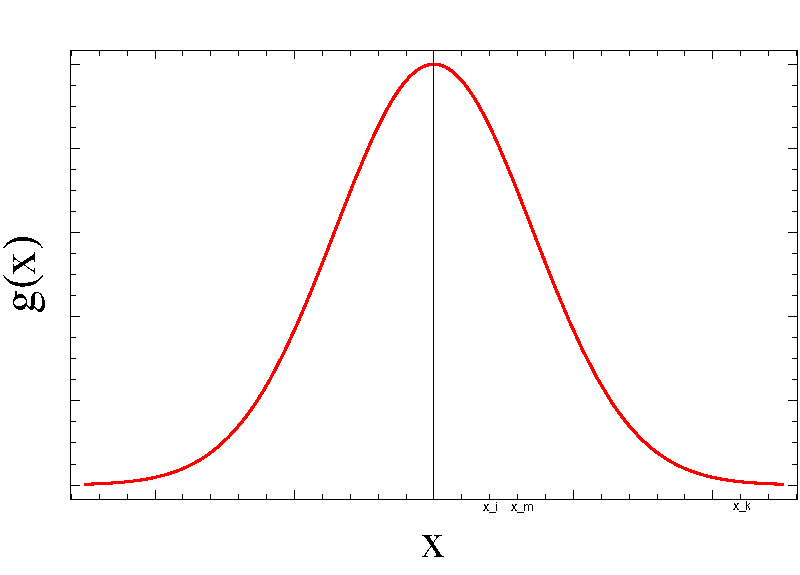
\includegraphics[scale=0.35]{distribution}
    \caption{Gaussian distribution showing problems in selection of random states}
    \label{fig:distribution}
\end{SCfigure}
\FloatBarrier
Preventing the simulation in creating biased averages and imprecise results is possible by using the Metropolis algorithm, which is a Markov process, satisfying both ergodicity and detailed balance.\\
Ergodicity in random processes means, that the time average of a sequence of events has to be the same as the average of all possible states, the so-called ensemble-average. In order to obey detailed balance, the process must follow a distribution, where the transition probability from state $i$ to state $j$ is the same as from state $j$ to state $i$ at equilibrium. This is also called reversibility.\\
Markov chains are referred to as random walks with selected probability to make a move, which is independent of the previous step. An example of this movement is the Brownian random walk shown in figure~\ref{fig:Brown}, where a particle moves in the $x$-$y$-plane with step length 1 preforming hundred steps. The probability of moving is the same for every direction. Using Markov processes, we can generate new random states and reach the most likely state (equilibrium) after a certain time.
\begin{SCfigure}[30][h]
    \centering
    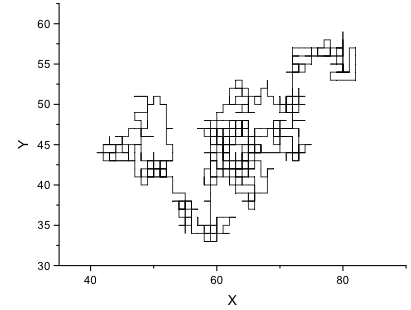
\includegraphics[scale=0.45]{Brown}
    \caption{Brownian random walk of 100 steps in $x$-$y$-plane and step length 1}
    \label{fig:Brown}
\end{SCfigure}
\FloatBarrier
In this report we have implemented the Metropolis test as following:
\begin{lstlisting}
// ----------------- metropolis test ---------------------------- //
if (ran2(&idum) <= wfnew*wfnew/wfold/wfold){
    for (j = 0; j < dimension; j++){
         r_old(i,j) = r_new(i,j);
         }
    wfold = wfnew;
    accept = accept + 1;
    }
}
\end{lstlisting}
where \texttt{wfnew} and \texttt{wfold} are the wave functions $\Psi(r_{old})$ and $\Psi(r_{new})$ and \texttt{ran2()} generates random numbers.\\
This means, that we test whether the random number is smaller, than the squared wave function at the new position divided by the squared wave function at the old position:
\begin{equation}
\texttt{ran2(\&idum)} <= q(r_{old},r_{new}) = \frac{\vert \psi_T(r_{new})\vert^2}{\vert \psi_T(r_{old})\vert ^2}
\end{equation}
\subsection{Importance sampling}\label{sec:importance}
There are lots of examples in science, where biasing is disturbing and should be avoided. One example are the required unbiased uncorrelated random numbers in section~\ref{sec:ran}. In Monte-carlo methods, biasing can be a tool to increase the simulation's efficiency by preforming a Metropolis walk biased by the trial wave function. Since our problem is somewhat simular to a diffusion process in one dimension for one particle, we may use an approach based on the Fokker-Planck and the Langevin equation.\\
The 'old' and 'new' positions in space can be caluclated by
\begin{align}
r_{old} &= \eta\\
r_{new} &= r_{old} + \eta + \delta t D F_{old},
\end{align}
where $\eta$ denotes a gaussian distributed random variable, $\delta t$ refers to the time step, $D$ is the diffusion constant, which is in our case set to $D=0.5$ and $F_{old}$ is the quantum force at position $r_{old}$. Note, that $\eta$ are different random numbers.\\
The term responsible for biasing the walk in space $x$ is the quantum force, which leads the walk to regions with large trial wave function. In a brute force Metropolis algorithm, the propability of moving would be the same for all directions. The quantum force is
\begin{align}\label{eq:quantum_force}
\mathbf{F}&= 2 \frac{1}{\psi_T} \mathbf{\nabla} \psi_T\\
&= 2 \left[|\mathbf{S\uparrow}(\alpha)||\mathbf{S\downarrow}(\alpha)|\prod_{i<j}^6 J(\beta)\right]^{-1} \mathbf{\nabla} \left(|\mathbf{S\uparrow}(\alpha)||\mathbf{S\downarrow}(\alpha)|\prod_{i<j}^6 J(\beta)\right).
\end{align}
In order to include this biasing in the Metropolis algorithm, we will replace
\begin{align}
q(r_{old},r_{new}) &= \frac{\vert \psi_T(r_{new})\vert^2}{\vert \psi_T(r_{old})\vert ^2}
\intertext{by}
q(r_{old},r_{new}) &= \frac{G(r_{old},r_{new},\delta t) \vert \psi_T(r_{new})\vert^2}{G(r_{new},r_{old},\delta t) \vert \psi_T(r_{old})\vert^2}, \label{glg:importance_s}
\intertext{where the quantity $G$ refers to the Greensfunction}
G(y,x,\delta t) &= \frac{1}{(4\pi D\delta t)^{3N/2}} \exp\left[-(y-x-D \delta t F(x))^2 \frac{1}{4D \delta t} \right]
\end{align}
In the source code this lookes like:
\begin{lstlisting}
// ----------------- metropolis test ---------------------------- //
if (ran2(&idum) <= greensfunction*wfnew*wfnew/wfold/wfold){
    for (j = 0; j < dimension; j++){
         r_old(i,j) = r_new(i,j);
         qforce_old(i,j) = qforce_new(i,j); 
         }
    wfold = wfnew;
    accept = accept + 1;
    }
}
\end{lstlisting}
Compared to the source code in section~\ref{sec:metropolis} we have just added to things: the additional \texttt{greensfunction} and the line, where we set \texttt{qforce\_old} to be \texttt{qforce\_new}. This is equivalent to what happens in equation~\ref{glg:importance_s}.


\subsection{Parallelization}
The code is parallelized with shared memory and realized through OpenMP. Every core goes thereby through the whole Monte-Carlo simulation and at the end the mean of the energies are taken. 


\subsection{Closed form solutions}\label{sec:closed_form}
The quantum force (eq. \ref{eq:quantum_force}) and the kinetic energy part in equation \ref{glg:localenergy} are until now calculated by a brute force derivation. A disadvantage of this method is, that the wavefunction has to be evaluated multiple times at different positions $r+h$, $r-h$ respectively. In order to optimize this step one can implement the analytical expressions. These are derived for example in \citet{hogberget2013}. The quantum force can thereby be expressed by
\begin{equation}
\mathbf{F_i} = 2 \left( \frac{\nabla_i |\mathbf{S\uparrow}|}{|\mathbf{S\uparrow}|} + \frac{\nabla_i J}{J} \right).
\end{equation}
The first part of the right side denotes the gradient of the Slater determinant, the second one the gradient of the Jastrow factor. It has to be payed attention that this is the expression for only one particle with index $i$ moved with spin up. Considering a spin down particle the $|\mathbf{S\uparrow}|$ becomes $|\mathbf{S\downarrow}|$. Further the kinetic part of the local energy arises as a result of
\begin{equation}
\frac{\nabla_i^2 \Psi_T}{\Psi_T} = \frac{\nabla_i^2 |\mathbf{S\uparrow}|}{|\mathbf{S\uparrow}|} + \frac{\nabla_i^2 J}{J} + 2\left( \frac{\nabla_i |\mathbf{S\uparrow}|}{|\mathbf{S\uparrow}|} \cdot \frac{\nabla_i J}{J} \right),
\end{equation}
again assuming a spin up particle.

The missing expressions can be obtained by deriving the trial wavefunction \ref{glg:sixelectron}. This is also done in \citet{hogberget2013} and reveals 
\begin{equation}\label{eq:jastrow-derivations}
    \frac{\nabla_i J}{J} = \sum_{k\neq i = 1}^{N}\frac{a_{ik}}{r_{ik}} \frac{\mathbf{r_i}-\mathbf{r_k}}{\left(1 + \beta r_{ik} \right)^2}
\end{equation}
for the gradient and 
\begin{equation}
    \frac{\nabla_i^2 J}{J} = \left| \frac{\nabla_i J}{J} \right| - \sum_{k\neq i = 1}^{N}a_{ik} \frac{\beta r_{ik} - 1}{r_{ik}\left(1 +\beta r_{ik} \right)^3} 
\end{equation}
for the laplacian of the Jastrow-factor. The derivations of the Slater determinants can be calculated to
\begin{equation}\label{eq:gradientslater}
    \frac{\nabla_i |\mathbf{S}|}{|\mathbf{S}|} = \sum_k \left( \nabla_i \phi_k(\mathbf{r}_i)\right)(\mathbf{S}_{ki}^{-1})
\end{equation}
for the gradient and
\begin{equation}\label{eq:laplacianslater}
    \frac{\nabla_i^2 |\mathbf{S}|}{|\mathbf{S}|} = \sum_k^{N/2} \left( \nabla_i^2 \phi_k(\mathbf{r}_i)\right)(\mathbf{S}_{ki}^{-1})
\end{equation}
for the laplacian. For the first part on the right side of eqs. \ref{eq:gradientslater} and \ref{eq:laplacianslater} exists analytical expressions which can be determined by applying the operands on the single particle equation \ref{glg:wavefunc1}. These can also be found in tabulated form in \citet[app. D]{hogberget2013}. The last term $\mathbf{S}_{ki}^{-1}$ is the transpose of the inverse Slater matrix. 